\section{User Study Results  (NEW VERSION!!!)}
\label{sec:results}

The next subsections present the results obtained.

\subsection{Participants}
\label{sec:results:participants}

The questionnaire was answered by $N = 31$ participants over a six-day window in May 2026. All responses were substantive, so no entries were removed during data cleaning. % The three figures that follow summarise the sample. Each is described in prose so the argument can be followed without consulting the chart.

Figure~\ref{fig:demographics-role-area} pairs the current role with the primary area of study or work. The role question allowed more than one selection, since some participants combine study and professional practice. Most respondents were students --- 16 undergraduates, 8 master's students, and 3 doctoral students. Four were professors or researchers. Five of the student respondents additionally reported professional experience outside the university; this appears in the role chart as a secondary multi-select pick rather than as a separate primary category. The area distribution is heavily skewed: 25 of the 31 participants come from Computer Science or Software Engineering, with 3 from Design or UX, 1 from Information Systems, and 2 from other technology areas.

\begin{figure}[ht]
\centering
\pdftooltip{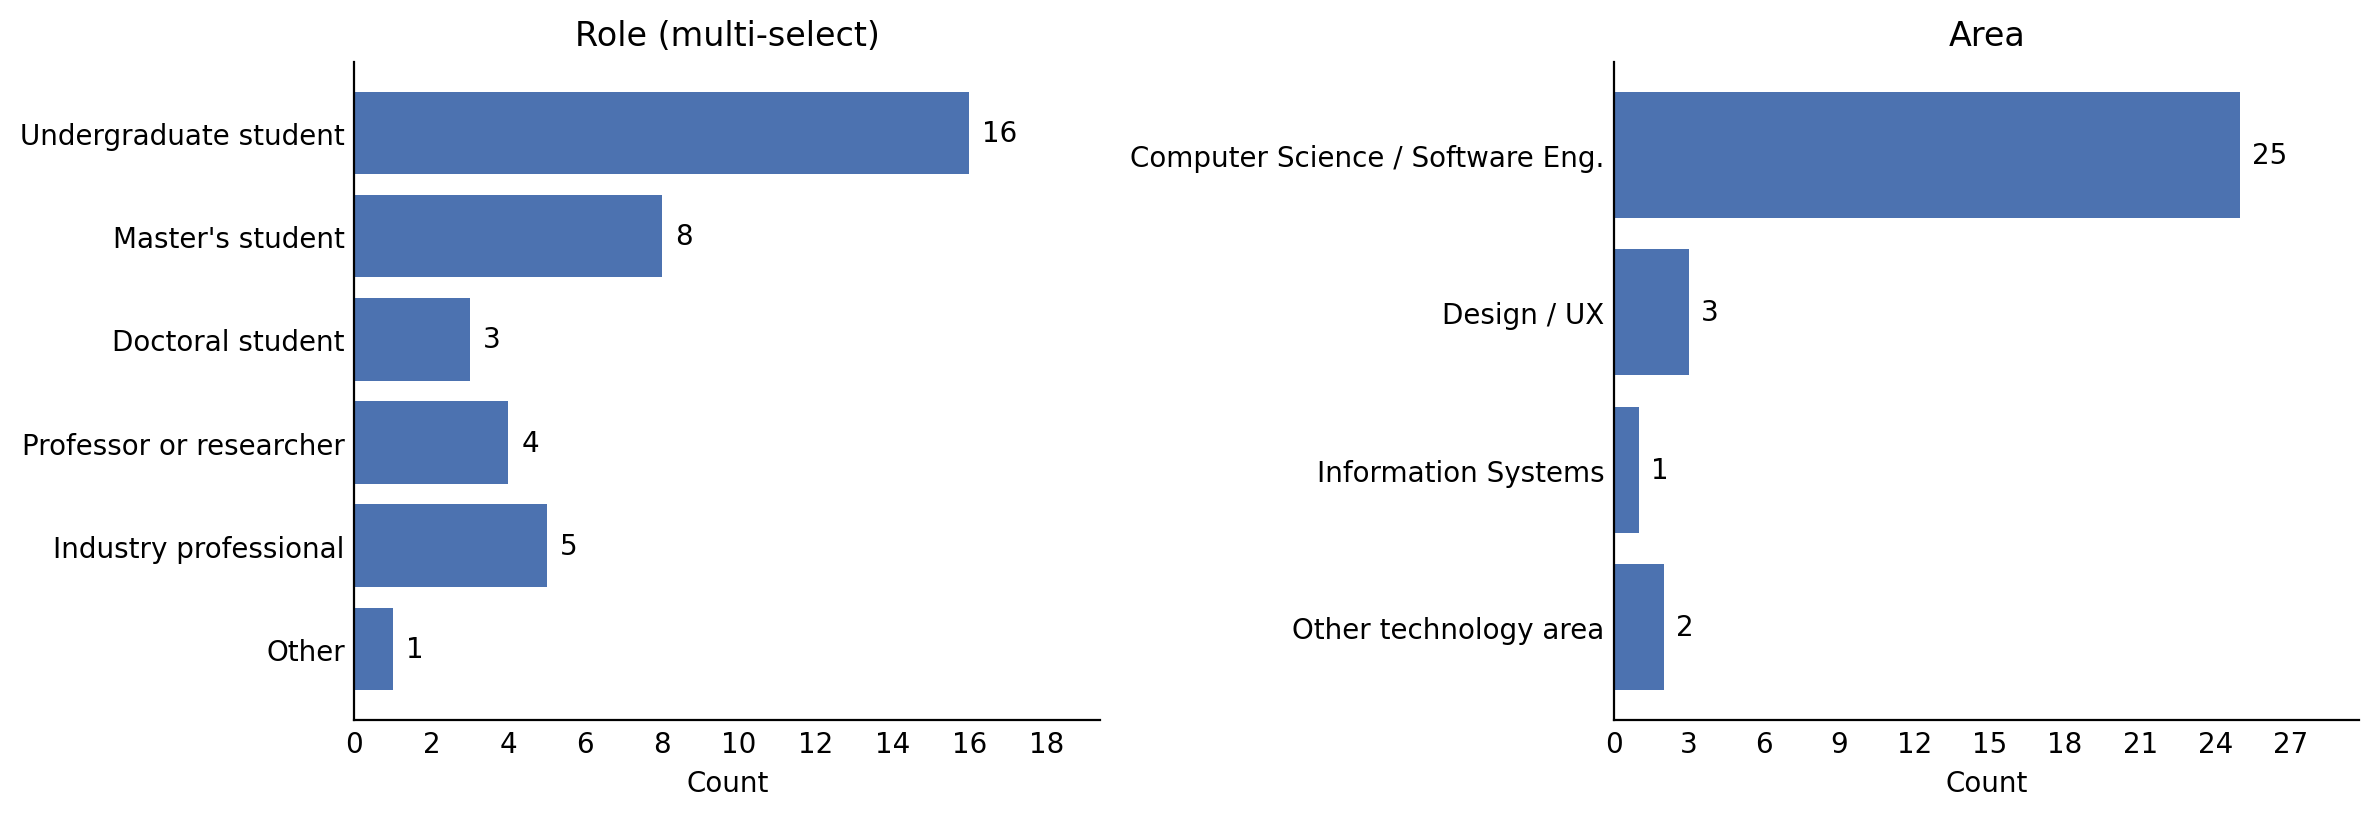
\includegraphics[width=.95\textwidth]{figures/demographics-role-area.png}}{Two horizontal bar charts side by side. The left chart shows the count of selections for each role option: 16 for undergraduate student, 8 for master's student, 3 for doctoral student, 4 for professor or researcher, 5 for industry professional, and 1 for ``other''. The role question was multi-select, so several participants selected more than one role; the ``industry professional'' count overlaps with student categories rather than denoting a separate primary group, and the total exceeds the sample size of 31. The right chart shows the count for each area: 25 for Computer Science or Software Engineering, 3 for Design or UX, 1 for Information Systems, and 2 for ``other technology area''.}
\caption{Participant roles (multi-select) and primary areas of study or work.}
\label{fig:demographics-role-area}
\end{figure}

Figure~\ref{fig:demographics-age} shows the age distribution. Ages span from 18 to 52, with a median of 24. Sixteen participants fall in the 18--24 range, 12 in the 25--34 range, 2 in the 35--44 range, and 1 in the 45--54 range. The sample skews young, which is consistent with the dominant student profile reported above.

\begin{figure}[ht]
\centering
\pdftooltip{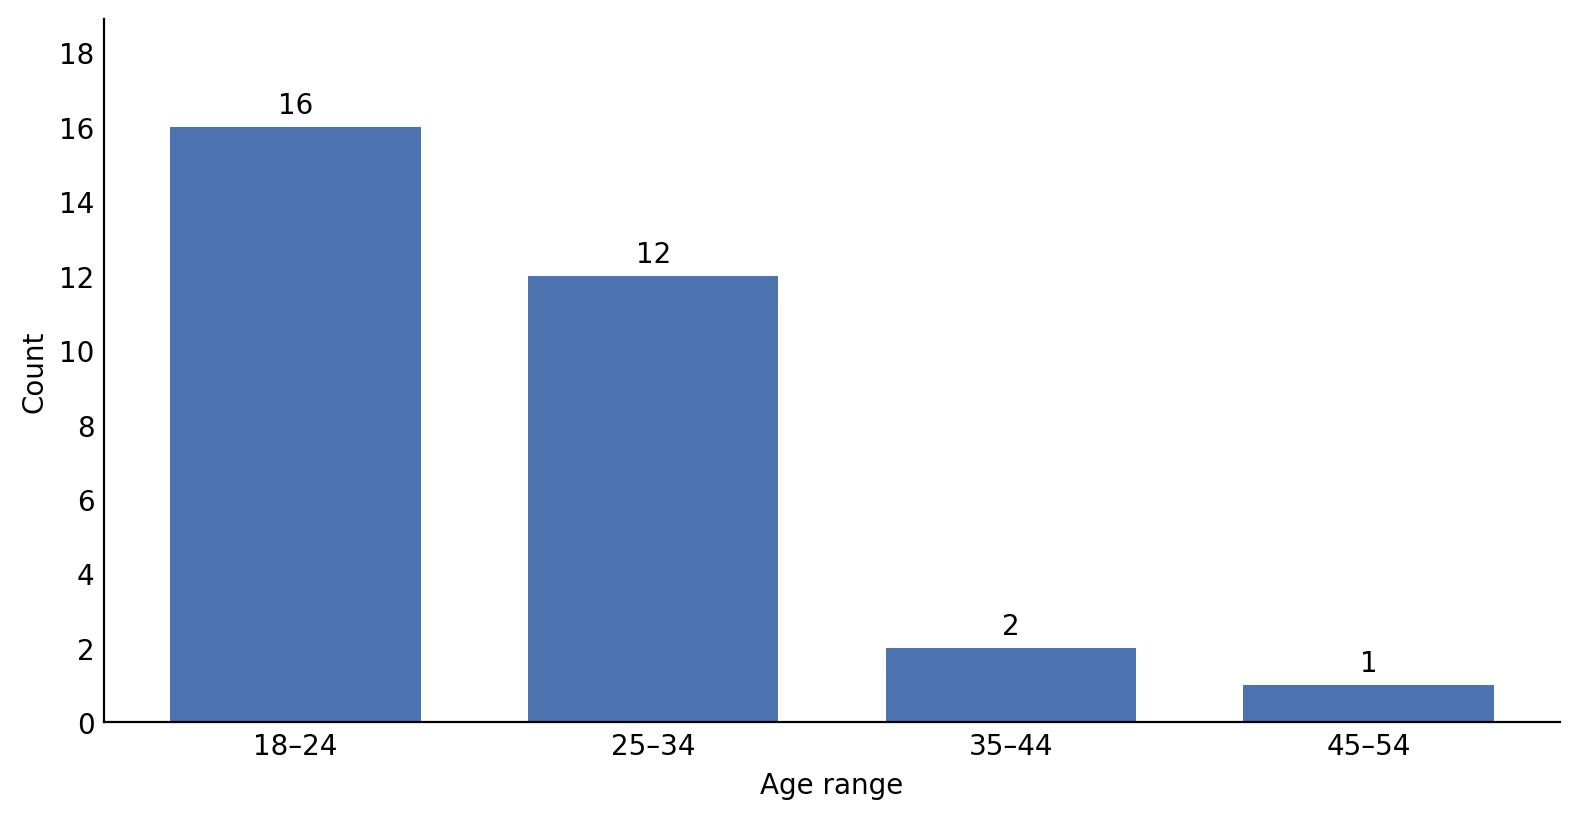
\includegraphics[width=.7\textwidth]{figures/demographics-age.png}}{A histogram of participant ages with four age-range bins on the horizontal axis: 18--24, 25--34, 35--44, and 45--54. The bars have heights 16, 12, 2, and 1, respectively. The distribution is right-skewed, with most participants in the youngest two bins.}
\caption{Distribution of participant ages across four age ranges.}
\label{fig:demographics-age}
\end{figure}

Figure~\ref{fig:expertise-profile} pairs prior familiarity with Nielsen's heuristics with practical experience in HCI or usability evaluation. Both scales are ordered from novice at the top to expert at the bottom. On the familiarity scale, 17 participants reported limited prior familiarity with the heuristics, 7 reported moderate familiarity, 6 knew them well, and 1 had already used them in projects or evaluations. On the practical-experience scale, 8 reported no practical experience, 13 reported little experience limited to coursework, 6 reported some experience in academic projects, and 4 reported regular practice in their professional or research work.

\begin{figure}[ht]
\centering
\pdftooltip{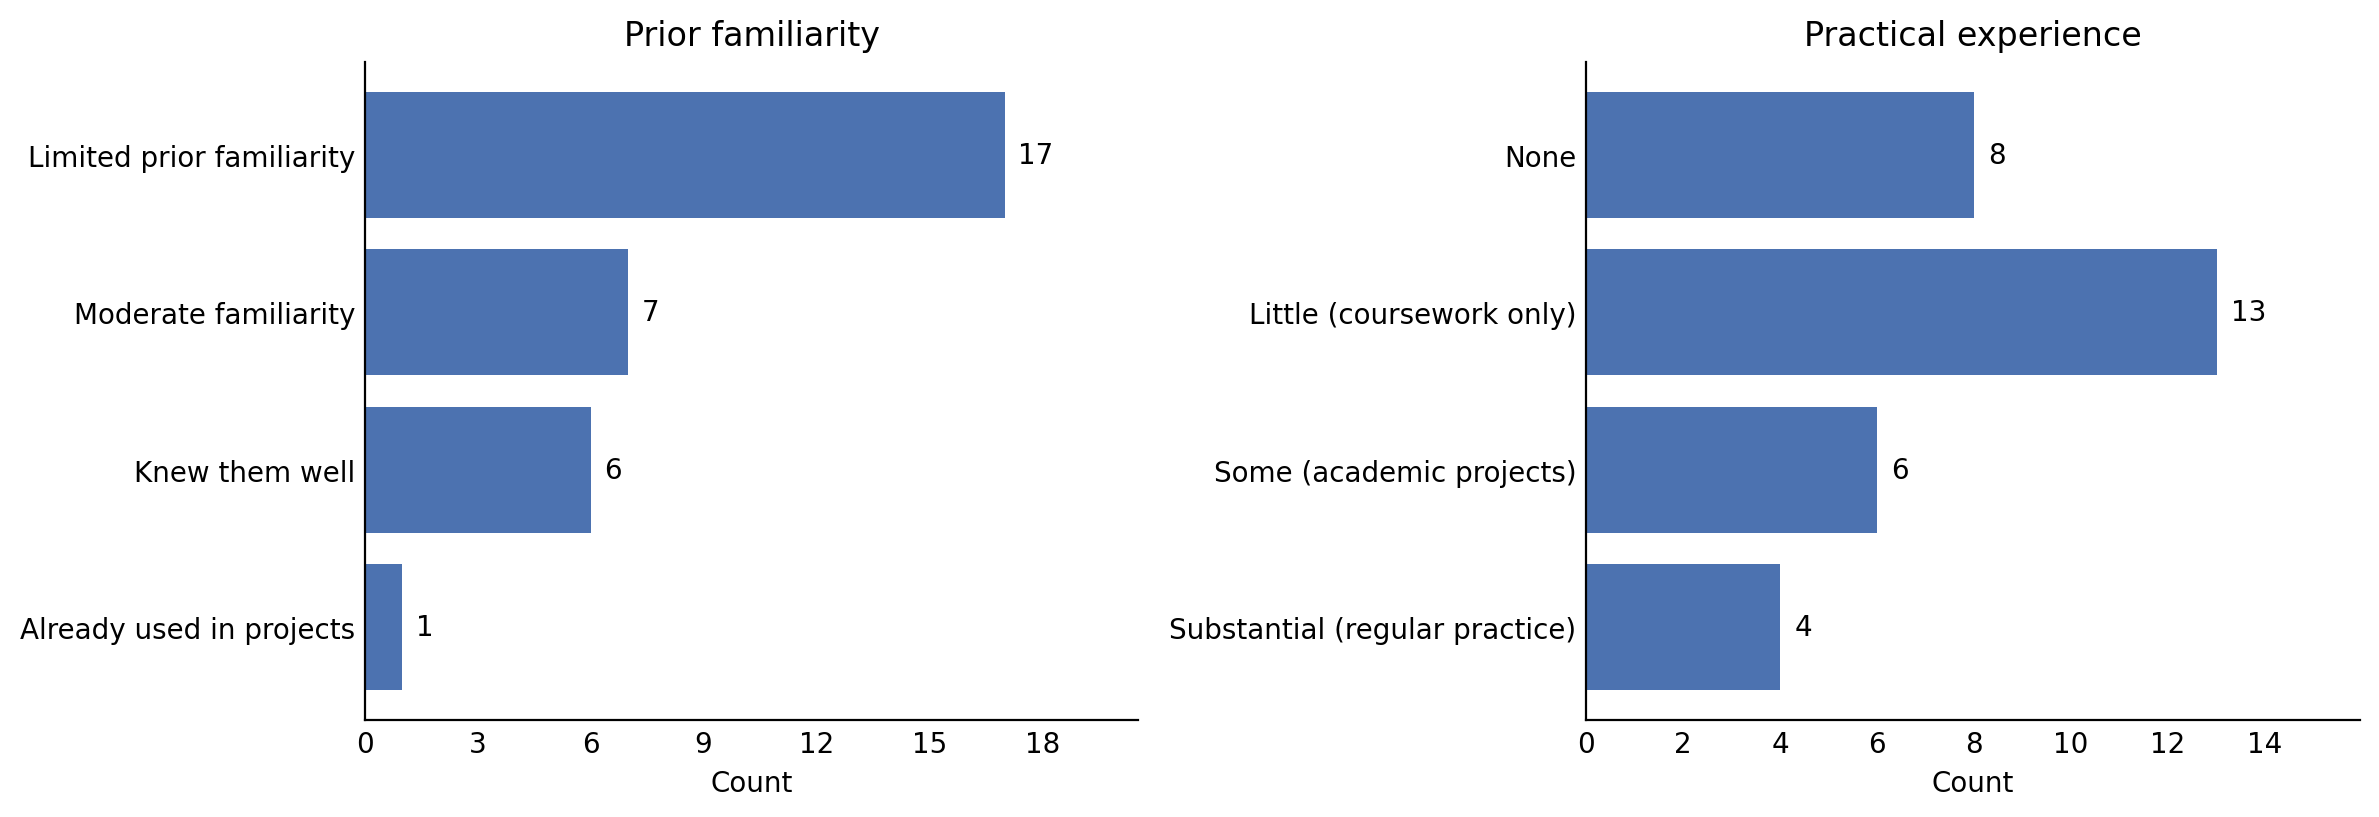
\includegraphics[width=.95\textwidth]{figures/expertise-profile.png}}{Two horizontal bar charts side by side, both ordered from novice at the top to expert at the bottom. The left chart shows the count for each level of prior familiarity with Nielsen's heuristics: 17 for ``limited prior familiarity'', 7 for ``moderate familiarity'', 6 for ``knew them well'', and 1 for ``had already used them in projects or evaluations''. The right chart shows the count for each level of practical experience with HCI or usability evaluation: 8 for ``none'', 13 for ``little, only in coursework'', 6 for ``some, in academic projects'', and 4 for ``substantial, in regular professional or research practice''.}
\caption{Prior familiarity with Nielsen's heuristics and practical experience with HCI or usability evaluation.}
\label{fig:expertise-profile}
\end{figure}

The sample is therefore dominated by computing students, most with limited prior familiarity with the heuristics. A smaller group --- designers, professors, and participants with more practical HCI experience --- provides a critical contrast in the qualitative analysis that follows. Participant identifiers ($P_1$ through $P_{31}$) are anonymous and follow the order in which the responses were received.\footnote{Original responses were written in Portuguese. Quotes shown in this section were translated by the authors; the AI-tool disclosure for translation is provided in the Acknowledgments.}

\subsection{Overall appreciation}
\label{sec:results:t1}

Most participants reported a positive overall experience with the game (27 of 31); the remaining four mixed or negative responses are revisited together in Section~\ref{sec:results:t6}. The reasons given for liking the game clustered into a few recurring themes.

The most common reason was \textbf{didactic clarity}. Several participants described the game as \textit{``didactic''} or \textit{``informative''}, and as a way to \textit{``transform theory into practice''} ($P_{19}$, undergraduate, Information Systems). A second recurring theme was that \textbf{the scenarios mirror real-world frustrations}. $P_1$ (master's, limited prior familiarity) noted that the game \textit{``showed problems that really happen and that companies do nothing to fix''}. $P_{16}$ (undergraduate, also industry professional) reframed this as a pedagogical strategy: \textit{``the game gives you a first-person perspective; suffering to learn is a good tactic so you do not make the same mistakes again''}.

\subsection{Perceived support for understanding}
\label{sec:results:t2}

When asked how the game supported their understanding of Nielsen's heuristics, participants identified three mechanisms that together account for most of the perceived support.

The first and most-cited mechanism is the \textbf{paired contrast} between the violating and the compliant scenarios. Nine participants named the contrast as the single most important aspect of the game. $P_1$ wrote that \textit{``the comparison between the examples was the most distinguishing feature; showing first the wrong version and then the right one helped me a lot''}. $P_{12}$ (master's, limited prior familiarity) made the same point in different words: \textit{``what helped me the most was the way the game first showed a messy scenario and right after a correct one''}. The same mechanism is named by $P_6$, $P_{11}$, $P_{15}$, $P_{16}$, $P_{21}$ and $P_{31}$, often using the words \textit{``error and correct''}, \textit{``worse versus better''}, or \textit{``without and with''} --- the same vocabulary the game itself uses on the reveal screen.

The second mechanism is the \textbf{interactive nature of the scenarios}. Participants treated \textit{``practical examples''} and \textit{``interactive interfaces''} as distinct from a static contrast: doing the task in the violating interface made the heuristic concrete. $P_{14}$ (professor, Design/UX, knew the heuristics well) summarized this clearly: \textit{``the fact that the interfaces are interactive contributed without doubt to a better understanding; it let me experience how the design is actually an obstacle for the user''}. $P_9$ (master's) gave the most specific illustration: ``the interactive part --- sending the message and feeling the impact of thinking it had been lost, for example''. The episode refers to the bad scenario for Heuristic~1 (Visibility of System Status), in which the player sends a message to a friend in an online chat and receives no feedback while the message is being sent. The same emphasis on interactivity as the source of understanding appears in $P_{10}$, $P_{13}$, $P_{17}$, $P_{22}$, $P_{23}$, and $P_{27}$.

The third mechanism is the \textbf{naming of the concept on the reveal screen}. For participants with limited prior familiarity with the heuristics, the reveal step is where the practical experience is named and labeled. $P_5$ (master's, limited prior familiarity) put it directly: \textit{``I did not even know these concepts had names like that''}. $P_{24}$ (undergraduate, also industry professional, moderate familiarity) added that \textit{``seeing each heuristic explained and named separately was useful; it added to what I already knew''}.

Several participants made the comparison with traditional reading explicit. $P_{30}$ articulated this most fully: \textit{``I would have taken longer to understand by reading a fancy definition on its own; this was a good combination of learning and entertainment. It is a more active method of learning than just reading, which is a more passive way.''} One participant offered a mild dissent: $P_7$, who did not find the game very supportive, still acknowledged that \textit{``at least we had some examples of errors and successes according to Nielsen's heuristics''}.

\subsection{Gamification and narration}
\label{sec:results:t3}

When asked about the effect of gamification (stars, progress bar, and the ``Heuristics Expert'' closing screen) and narration on their experience and learning, participants' responses split cleanly into two sub-themes, which we present separately because the responses diverge in direction.

For \textbf{gamification}, thirteen participants reported a positive effect on focus or motivation. $P_1$ noted that the gamification \textit{``helped me stay focused and more immersed; it stopped being something boring and only theoretical''}. $P_{24}$ added that \textit{``gamifying helped me hold my attention and made the learning process more satisfying''}. A separate group of six respondents singled out the progress bar as helpful while saying the stars and the Expert screen did not affect them. $P_2$ wrote that \textit{``the progress bar gave me a sense of arriving somewhere; the stars did not influence me or motivate me''}. $P_{31}$ gave the underlying reason: \textit{``I liked the progress bar; I hate it when something does not tell you how long it will be and seems to never end''}, framing the bar as a defense against the experience of an open-ended task. Three participants reported no effect from gamification at all ($P_{13}$, $P_{29}$, $P_{30}$). The remaining critique was structural: $P_6$ (professor) said gamification \textit{``helped only superficially, since there was practically only one path to follow and it was not possible to lose points''}; $P_7$ extended this into a call for \textit{``a real gamification with scoring and rewards''}.

For \textbf{narration}, ten participants described it as helping them focus or recognise the heuristic in action. $P_8$ (master's, limited prior familiarity) gave the sharpest example: \textit{``in some cases without the heuristic I got irritated by the lack of pattern, and the narration helped me understand that this was exactly what was being demonstrated''}. $P_{14}$ added that \textit{``the narration contributed to understanding and to staying focused on the activity''}. $P_{31}$ named a distinct mechanism --- the narration as a way of taking the reading work off the player so they can engage with the practical task: \textit{``the most interesting part for me was the narration; constantly reading non-practical aspects makes you feel lazy when you have to start doing something practical, and having the narrator do that work brings down a barrier so you can focus on what matters''}. Four participants reported the opposite effect. $P_{18}$ wrote that the narration \textit{``bothered me a bit''} and that a button to silence it was missing; $P_{20}$ and $P_{22}$ raised similar points about volume control and distraction from reading. $P_{10}$ accepted the narration but commented that it \textit{``could be a little less robotic''}.

\subsection{Reported issues and suggestions}
\label{sec:results:t4}

When asked about negative points and improvements, and in optional general comments at the end of the questionnaire, three recurring patterns appear across the responses.

The most consistent pattern is a \textbf{wish for the player to be able to fail or to choose}. Five participants asked for an explicit way to be wrong or for more challenge. $P_2$ suggested that the user should try to identify which heuristic applies before the game reveals it; $P_7$ argued that without the possibility of error there is no need to reason, which makes the experience tedious; $P_8$ proposed losing stars or lives on mistakes; $P_{18}$ and $P_{25}$ asked for a more interactive format with real decisions. The wording differs but the underlying request is the same: a recognition step that the player completes before the reveal screen.

The second pattern is \textbf{narration ergonomics}. Beyond the mixed reception reported in Section~\ref{sec:results:t3}, four participants pointed to concrete affordances: $P_5$ asked that the audio not play automatically; $P_{18}$ and $P_{20}$ asked for a mute or volume control; $P_9$ noted that some narration tracks were long enough to feel like watching a video. These are inexpensive to address.

The third pattern is a \textbf{desire for more depth} and a small set of one-off suggestions. $P_{16}$ proposed adding a second activity per heuristic to support fixation and $P_6$ suggested that some scenarios could be replaced by more realistic variants. A scattered set of further comments touched on small interface details and atmosphere --- including $P_{17}$'s suggestion that the game open with a light-hearted warning about being intentionally frustrating at first --- but did not cluster within a shared theme.

\subsection{Critical reception}
\label{sec:results:t6}

Four of the thirty-one responses read the artefact more as a guided demonstration than as a game proper. The three quoted below illustrate the range of how this position was expressed. $P_2$ (master's, designer, knew the heuristics well) expected to be challenged and instead experienced \textit{``almost a guided tour through the heuristics''}. $P_7$ (undergraduate) was more explicit: \textit{``there is no aspect of it that resembles a game''}, because \textit{``the user cannot make mistakes and there is no incentive to reason about the answer''}. $P_{30}$ (undergraduate, limited prior familiarity) reached the same conclusion through a different route: \textit{``as a game, no --- in my experience this is a demonstration of how user experience can be done badly, and the corresponding solutions''}.

We return to this tension, and to the related calls for a recognition step or a scoring layer surfaced in Section~\ref{sec:results:t4}, in the discussion of theme 4 in Section~\ref{sec:discussion}.
